

\tikzset{every picture/.style={line width=0.75pt}} %set default line width to 0.75pt        

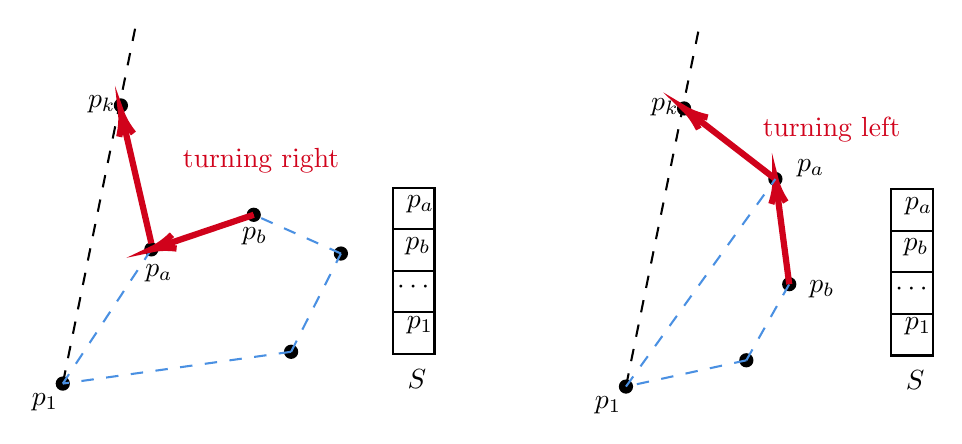
\begin{tikzpicture}[x=0.5pt,y=0.5pt,yscale=-1,xscale=1]
%uncomment if require: \path (0,384); %set diagram left start at 0, and has height of 384

%Flowchart: Connector [id:dp3291568735294871] 
\draw  [fill={rgb, 255:red, 0; green, 0; blue, 0 }  ,fill opacity=1 ] (78,116) .. controls (78,113.58) and (79.96,111.62) .. (82.38,111.62) .. controls (84.79,111.62) and (86.75,113.58) .. (86.75,116) .. controls (86.75,118.42) and (84.79,120.38) .. (82.38,120.38) .. controls (79.96,120.38) and (78,118.42) .. (78,116) -- cycle ;
%Flowchart: Connector [id:dp6621594719883535] 
\draw  [fill={rgb, 255:red, 0; green, 0; blue, 0 }  ,fill opacity=1 ] (201,294) .. controls (201,291.58) and (202.96,289.62) .. (205.38,289.62) .. controls (207.79,289.62) and (209.75,291.58) .. (209.75,294) .. controls (209.75,296.42) and (207.79,298.38) .. (205.38,298.38) .. controls (202.96,298.38) and (201,296.42) .. (201,294) -- cycle ;
%Flowchart: Connector [id:dp25920829224973985] 
\draw  [fill={rgb, 255:red, 0; green, 0; blue, 0 }  ,fill opacity=1 ] (36,317) .. controls (36,314.58) and (37.96,312.62) .. (40.38,312.62) .. controls (42.79,312.62) and (44.75,314.58) .. (44.75,317) .. controls (44.75,319.42) and (42.79,321.38) .. (40.38,321.38) .. controls (37.96,321.38) and (36,319.42) .. (36,317) -- cycle ;
%Flowchart: Connector [id:dp23175126343110752] 
\draw  [fill={rgb, 255:red, 0; green, 0; blue, 0 }  ,fill opacity=1 ] (100,220) .. controls (100,217.58) and (101.96,215.62) .. (104.38,215.62) .. controls (106.79,215.62) and (108.75,217.58) .. (108.75,220) .. controls (108.75,222.42) and (106.79,224.38) .. (104.38,224.38) .. controls (101.96,224.38) and (100,222.42) .. (100,220) -- cycle ;
%Flowchart: Connector [id:dp226256241933963] 
\draw  [fill={rgb, 255:red, 0; green, 0; blue, 0 }  ,fill opacity=1 ] (237,223) .. controls (237,220.58) and (238.96,218.62) .. (241.38,218.62) .. controls (243.79,218.62) and (245.75,220.58) .. (245.75,223) .. controls (245.75,225.42) and (243.79,227.38) .. (241.38,227.38) .. controls (238.96,227.38) and (237,225.42) .. (237,223) -- cycle ;
%Straight Lines [id:da8400967027516107] 
\draw [color={rgb, 255:red, 74; green, 144; blue, 226 }  ,draw opacity=1 ] [dash pattern={on 4.5pt off 4.5pt}]  (205.38,294) -- (40.38,317) ;
%Straight Lines [id:da44754220202255635] 
\draw  [dash pattern={on 4.5pt off 4.5pt}]  (92.63,60.52) -- (40.38,317) ;
%Flowchart: Connector [id:dp1733314058116755] 
\draw  [fill={rgb, 255:red, 0; green, 0; blue, 0 }  ,fill opacity=1 ] (174,195) .. controls (174,192.58) and (175.96,190.62) .. (178.38,190.62) .. controls (180.79,190.62) and (182.75,192.58) .. (182.75,195) .. controls (182.75,197.42) and (180.79,199.38) .. (178.38,199.38) .. controls (175.96,199.38) and (174,197.42) .. (174,195) -- cycle ;
%Straight Lines [id:da6595200138207884] 
\draw [color={rgb, 255:red, 74; green, 144; blue, 226 }  ,draw opacity=1 ] [dash pattern={on 4.5pt off 4.5pt}]  (104.38,220) -- (40.38,317) ;
%Straight Lines [id:da7758013938241641] 
\draw [color={rgb, 255:red, 208; green, 2; blue, 27 }  ,draw opacity=1 ] [dash pattern={on 4.5pt off 4.5pt}]  (178.38,195) -- (104.38,220) ;
%Straight Lines [id:da3686871889066282] 
\draw [color={rgb, 255:red, 74; green, 144; blue, 226 }  ,draw opacity=1 ] [dash pattern={on 4.5pt off 4.5pt}]  (241.38,223) -- (178.38,195) ;
%Straight Lines [id:da610731396524822] 
\draw [color={rgb, 255:red, 74; green, 144; blue, 226 }  ,draw opacity=1 ] [dash pattern={on 4.5pt off 4.5pt}]  (205.38,294) -- (241.38,223) ;
%Shape: Grid [id:dp4209096809685794] 
\draw  [draw opacity=0] (279,175.52) -- (309,175.52) -- (309,295.52) -- (279,295.52) -- cycle ; \draw    ; \draw   (279,205.52) -- (309,205.52)(279,235.52) -- (309,235.52)(279,265.52) -- (309,265.52) ; \draw   (279,175.52) -- (309,175.52) -- (309,295.52) -- (279,295.52) -- cycle ;
%Straight Lines [id:da9339984766179712] 
\draw [color={rgb, 255:red, 208; green, 2; blue, 27 }  ,draw opacity=1 ][line width=2.25]    (104.38,215.62) -- (83.28,124.27) ;
\draw [shift={(82.38,120.38)}, rotate = 436.99] [color={rgb, 255:red, 208; green, 2; blue, 27 }  ,draw opacity=1 ][line width=2.25]    (17.49,-5.26) .. controls (11.12,-2.23) and (5.29,-0.48) .. (0,0) .. controls (5.29,0.48) and (11.12,2.23) .. (17.49,5.26)   ;
%Straight Lines [id:da3526208773719812] 
\draw [color={rgb, 255:red, 208; green, 2; blue, 27 }  ,draw opacity=1 ][line width=2.25]    (178.38,195) -- (108.17,218.72) ;
\draw [shift={(104.38,220)}, rotate = 341.33000000000004] [color={rgb, 255:red, 208; green, 2; blue, 27 }  ,draw opacity=1 ][line width=2.25]    (17.49,-5.26) .. controls (11.12,-2.23) and (5.29,-0.48) .. (0,0) .. controls (5.29,0.48) and (11.12,2.23) .. (17.49,5.26)   ;
%Flowchart: Connector [id:dp777655020217685] 
\draw  [fill={rgb, 255:red, 0; green, 0; blue, 0 }  ,fill opacity=1 ] (485,118.15) .. controls (485,115.73) and (486.96,113.77) .. (489.38,113.77) .. controls (491.79,113.77) and (493.75,115.73) .. (493.75,118.15) .. controls (493.75,120.56) and (491.79,122.52) .. (489.38,122.52) .. controls (486.96,122.52) and (485,120.56) .. (485,118.15) -- cycle ;
%Flowchart: Connector [id:dp9509940585964177] 
\draw  [fill={rgb, 255:red, 0; green, 0; blue, 0 }  ,fill opacity=1 ] (530,300.15) .. controls (530,297.73) and (531.96,295.77) .. (534.38,295.77) .. controls (536.79,295.77) and (538.75,297.73) .. (538.75,300.15) .. controls (538.75,302.56) and (536.79,304.52) .. (534.38,304.52) .. controls (531.96,304.52) and (530,302.56) .. (530,300.15) -- cycle ;
%Flowchart: Connector [id:dp13535258001392825] 
\draw  [fill={rgb, 255:red, 0; green, 0; blue, 0 }  ,fill opacity=1 ] (443,319.15) .. controls (443,316.73) and (444.96,314.77) .. (447.38,314.77) .. controls (449.79,314.77) and (451.75,316.73) .. (451.75,319.15) .. controls (451.75,321.56) and (449.79,323.52) .. (447.38,323.52) .. controls (444.96,323.52) and (443,321.56) .. (443,319.15) -- cycle ;
%Flowchart: Connector [id:dp01259787733434159] 
\draw  [fill={rgb, 255:red, 0; green, 0; blue, 0 }  ,fill opacity=1 ] (551,169.15) .. controls (551,166.73) and (552.96,164.77) .. (555.38,164.77) .. controls (557.79,164.77) and (559.75,166.73) .. (559.75,169.15) .. controls (559.75,171.56) and (557.79,173.52) .. (555.38,173.52) .. controls (552.96,173.52) and (551,171.56) .. (551,169.15) -- cycle ;
%Straight Lines [id:da6618567782842074] 
\draw [color={rgb, 255:red, 74; green, 144; blue, 226 }  ,draw opacity=1 ] [dash pattern={on 4.5pt off 4.5pt}]  (534.38,300.15) -- (447.38,319.15) ;
%Straight Lines [id:da16840703639725407] 
\draw  [dash pattern={on 4.5pt off 4.5pt}]  (499.63,62.67) -- (447.38,319.15) ;
%Flowchart: Connector [id:dp28567136793902825] 
\draw  [fill={rgb, 255:red, 0; green, 0; blue, 0 }  ,fill opacity=1 ] (561,245.15) .. controls (561,242.73) and (562.96,240.77) .. (565.38,240.77) .. controls (567.79,240.77) and (569.75,242.73) .. (569.75,245.15) .. controls (569.75,247.56) and (567.79,249.52) .. (565.38,249.52) .. controls (562.96,249.52) and (561,247.56) .. (561,245.15) -- cycle ;
%Straight Lines [id:da795218588512217] 
\draw [color={rgb, 255:red, 74; green, 144; blue, 226 }  ,draw opacity=1 ] [dash pattern={on 4.5pt off 4.5pt}]  (555.38,169.15) -- (565.38,240.77) ;
%Straight Lines [id:da8869217620231401] 
\draw [color={rgb, 255:red, 74; green, 144; blue, 226 }  ,draw opacity=1 ] [dash pattern={on 4.5pt off 4.5pt}]  (534.38,300.15) -- (565.38,245.15) ;
%Shape: Grid [id:dp22696195921051476] 
\draw  [draw opacity=0] (639,176.67) -- (669,176.67) -- (669,296.67) -- (639,296.67) -- cycle ; \draw    ; \draw   (639,206.67) -- (669,206.67)(639,236.67) -- (669,236.67)(639,266.67) -- (669,266.67) ; \draw   (639,176.67) -- (669,176.67) -- (669,296.67) -- (639,296.67) -- cycle ;
%Straight Lines [id:da10377189210248139] 
\draw [color={rgb, 255:red, 208; green, 2; blue, 27 }  ,draw opacity=1 ][line width=2.25]    (565.38,245.15) -- (555.9,173.11) ;
\draw [shift={(555.38,169.15)}, rotate = 442.5] [color={rgb, 255:red, 208; green, 2; blue, 27 }  ,draw opacity=1 ][line width=2.25]    (17.49,-5.26) .. controls (11.12,-2.23) and (5.29,-0.48) .. (0,0) .. controls (5.29,0.48) and (11.12,2.23) .. (17.49,5.26)   ;
%Straight Lines [id:da44393308824629707] 
\draw [color={rgb, 255:red, 208; green, 2; blue, 27 }  ,draw opacity=1 ][line width=2.25]    (555.38,169.15) -- (492.54,120.59) ;
\draw [shift={(489.38,118.15)}, rotate = 397.69] [color={rgb, 255:red, 208; green, 2; blue, 27 }  ,draw opacity=1 ][line width=2.25]    (17.49,-5.26) .. controls (11.12,-2.23) and (5.29,-0.48) .. (0,0) .. controls (5.29,0.48) and (11.12,2.23) .. (17.49,5.26)   ;
%Straight Lines [id:da7079759298622591] 
\draw [color={rgb, 255:red, 74; green, 144; blue, 226 }  ,draw opacity=1 ] [dash pattern={on 4.5pt off 4.5pt}]  (447.38,319.15) -- (555.38,169.15) ;

% Text Node
\draw (97.75,228.93) node [anchor=north west][inner sep=0.75pt]   [align=left] {$\displaystyle p_{a}$};
% Text Node
\draw (15.75,321.93) node [anchor=north west][inner sep=0.75pt]   [align=left] {$\displaystyle p_{1}$};
% Text Node
\draw (167.75,201.93) node [anchor=north west][inner sep=0.75pt]   [align=left] {$\displaystyle p_{b}$};
% Text Node
\draw (56.38,106.31) node [anchor=north west][inner sep=0.75pt]   [align=left] {$\displaystyle p_{k}$};
% Text Node
\draw (286.75,178.93) node [anchor=north west][inner sep=0.75pt]   [align=left] {$\displaystyle p_{a}$};
% Text Node
\draw (285.75,208.93) node [anchor=north west][inner sep=0.75pt]   [align=left] {$\displaystyle p_{b}$};
% Text Node
\draw (279.75,240.93) node [anchor=north west][inner sep=0.75pt]   [align=left] {$\displaystyle \cdots $};
% Text Node
\draw (286.75,266.08) node [anchor=north west][inner sep=0.75pt]   [align=left] {$\displaystyle p_{1}$};
% Text Node
\draw (287.38,304.31) node [anchor=north west][inner sep=0.75pt]   [align=left] {$\displaystyle S$};
% Text Node
\draw (125,144.93) node [anchor=north west][inner sep=0.75pt]   [align=left] {\textcolor[rgb]{0.82,0.01,0.11}{turning right}};
% Text Node
\draw (568.75,153.08) node [anchor=north west][inner sep=0.75pt]   [align=left] {$\displaystyle p_{a}$};
% Text Node
\draw (422.75,324.08) node [anchor=north west][inner sep=0.75pt]   [align=left] {$\displaystyle p_{1}$};
% Text Node
\draw (577.75,240.08) node [anchor=north west][inner sep=0.75pt]   [align=left] {$\displaystyle p_{b}$};
% Text Node
\draw (463.38,108.46) node [anchor=north west][inner sep=0.75pt]   [align=left] {$\displaystyle p_{k}$};
% Text Node
\draw (646.75,180.08) node [anchor=north west][inner sep=0.75pt]   [align=left] {$\displaystyle p_{a}$};
% Text Node
\draw (645.75,210.08) node [anchor=north west][inner sep=0.75pt]   [align=left] {$\displaystyle p_{b}$};
% Text Node
\draw (639.75,242.08) node [anchor=north west][inner sep=0.75pt]   [align=left] {$\displaystyle \cdots $};
% Text Node
\draw (646.75,267.23) node [anchor=north west][inner sep=0.75pt]   [align=left] {$\displaystyle p_{1}$};
% Text Node
\draw (647.38,305.46) node [anchor=north west][inner sep=0.75pt]   [align=left] {$\displaystyle S$};
% Text Node
\draw (544,122.08) node [anchor=north west][inner sep=0.75pt]   [align=left] {\textcolor[rgb]{0.82,0.01,0.11}{turning left}};


\end{tikzpicture}

